% generated by gen_mem_fig.py -- do not edit by hand
\documentclass[10pt]{standalone}
\usepackage{helvet}
\renewcommand{\familydefault}{\sfdefault}
\usepackage{amsmath,amssymb}
\usepackage{tikz}
\usetikzlibrary{arrows.meta,patterns}
\definecolor{cctrl}{HTML}{D6E0EC}
\definecolor{cctrlb}{HTML}{3B5675}
\definecolor{cmem}{HTML}{FBE5D6}
\definecolor{cmemb}{HTML}{C55A11}
\definecolor{cA}{HTML}{CFE2F3}
\definecolor{cB}{HTML}{FCE5CD}
\definecolor{cC}{HTML}{D9EAD3}
\definecolor{cD}{HTML}{EAD1DC}
\newcommand{\fs}{\fontsize{6.4}{7.4}\selectfont}
\newcommand{\fss}{\fontsize{5.8}{6.6}\selectfont}
\begin{document}
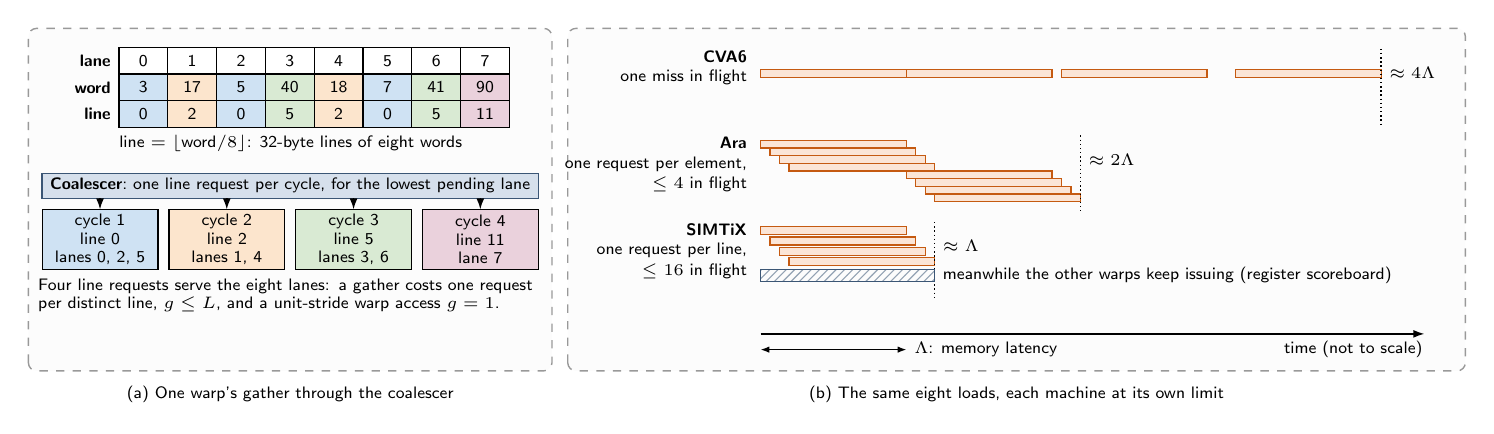
\begin{tikzpicture}[x=1cm, y=1cm,
  base/.style={align=center, font=\fs, inner sep=1pt, line width=0.5pt},
  ctrl/.style={base, draw=cctrlb, fill=cctrl},
  tbl/.style={draw=black, line width=0.45pt},
  cell/.style={font=\fss, inner sep=0.5pt}, cellh/.style={font=\fss\bfseries, inner sep=0.5pt},
  panel/.style={draw=black!40, dashed, rounded corners=3pt, fill=black!1, line width=0.5pt},
  lbl/.style={font=\fs, inner sep=0.5pt},
  note/.style={font=\fss, inner sep=0.5pt, align=left},
  subcap/.style={font=\fs, inner sep=1pt},
  bar/.style={draw=cmemb, fill=cmem, line width=0.45pt},
  arr/.style={-{Latex[length=1.4mm, width=1.0mm]}, line width=0.55pt}]

\draw[panel] (-0.100,-0.050) rectangle (6.550,4.300);
\node[cellh, anchor=east] at (0.970,3.890) {lane};
\node[cellh, anchor=east] at (0.970,3.550) {word};
\node[cellh, anchor=east] at (0.970,3.210) {line};
\draw[tbl, fill=white] (1.050,3.720) rectangle (1.670,4.060);
\node[cell] at (1.360,3.890) {0};
\draw[tbl, fill=cA] (1.050,3.380) rectangle (1.670,3.720);
\node[cell] at (1.360,3.550) {3};
\draw[tbl, fill=cA] (1.050,3.040) rectangle (1.670,3.380);
\node[cell] at (1.360,3.210) {0};
\draw[tbl, fill=white] (1.670,3.720) rectangle (2.290,4.060);
\node[cell] at (1.980,3.890) {1};
\draw[tbl, fill=cB] (1.670,3.380) rectangle (2.290,3.720);
\node[cell] at (1.980,3.550) {17};
\draw[tbl, fill=cB] (1.670,3.040) rectangle (2.290,3.380);
\node[cell] at (1.980,3.210) {2};
\draw[tbl, fill=white] (2.290,3.720) rectangle (2.910,4.060);
\node[cell] at (2.600,3.890) {2};
\draw[tbl, fill=cA] (2.290,3.380) rectangle (2.910,3.720);
\node[cell] at (2.600,3.550) {5};
\draw[tbl, fill=cA] (2.290,3.040) rectangle (2.910,3.380);
\node[cell] at (2.600,3.210) {0};
\draw[tbl, fill=white] (2.910,3.720) rectangle (3.530,4.060);
\node[cell] at (3.220,3.890) {3};
\draw[tbl, fill=cC] (2.910,3.380) rectangle (3.530,3.720);
\node[cell] at (3.220,3.550) {40};
\draw[tbl, fill=cC] (2.910,3.040) rectangle (3.530,3.380);
\node[cell] at (3.220,3.210) {5};
\draw[tbl, fill=white] (3.530,3.720) rectangle (4.150,4.060);
\node[cell] at (3.840,3.890) {4};
\draw[tbl, fill=cB] (3.530,3.380) rectangle (4.150,3.720);
\node[cell] at (3.840,3.550) {18};
\draw[tbl, fill=cB] (3.530,3.040) rectangle (4.150,3.380);
\node[cell] at (3.840,3.210) {2};
\draw[tbl, fill=white] (4.150,3.720) rectangle (4.770,4.060);
\node[cell] at (4.460,3.890) {5};
\draw[tbl, fill=cA] (4.150,3.380) rectangle (4.770,3.720);
\node[cell] at (4.460,3.550) {7};
\draw[tbl, fill=cA] (4.150,3.040) rectangle (4.770,3.380);
\node[cell] at (4.460,3.210) {0};
\draw[tbl, fill=white] (4.770,3.720) rectangle (5.390,4.060);
\node[cell] at (5.080,3.890) {6};
\draw[tbl, fill=cC] (4.770,3.380) rectangle (5.390,3.720);
\node[cell] at (5.080,3.550) {41};
\draw[tbl, fill=cC] (4.770,3.040) rectangle (5.390,3.380);
\node[cell] at (5.080,3.210) {5};
\draw[tbl, fill=white] (5.390,3.720) rectangle (6.010,4.060);
\node[cell] at (5.700,3.890) {7};
\draw[tbl, fill=cD] (5.390,3.380) rectangle (6.010,3.720);
\node[cell] at (5.700,3.550) {90};
\draw[tbl, fill=cD] (5.390,3.040) rectangle (6.010,3.380);
\node[cell] at (5.700,3.210) {11};
\node[note, anchor=north west] at (1.030,2.970) {line $=\lfloor \text{word}/8\rfloor$: 32-byte lines of eight words};
\node[ctrl, minimum width=6.30cm, minimum height=0.32cm] at (3.225,2.300) {\textbf{Coalescer}:\ \fss one line request per cycle, for the lowest pending lane};
\draw[arr] (0.810,2.140) -- (0.810,2.000);
\draw[tbl, fill=cA] (0.075,1.240) rectangle (1.545,2.000);
\node[cell, align=center] at (0.810,1.620) {cycle 1\\line 0\\lanes 0, 2, 5};
\draw[arr] (2.420,2.140) -- (2.420,2.000);
\draw[tbl, fill=cB] (1.685,1.240) rectangle (3.155,2.000);
\node[cell, align=center] at (2.420,1.620) {cycle 2\\line 2\\lanes 1, 4};
\draw[arr] (4.030,2.140) -- (4.030,2.000);
\draw[tbl, fill=cC] (3.295,1.240) rectangle (4.765,2.000);
\node[cell, align=center] at (4.030,1.620) {cycle 3\\line 5\\lanes 3, 6};
\draw[arr] (5.640,2.140) -- (5.640,2.000);
\draw[tbl, fill=cD] (4.905,1.240) rectangle (6.375,2.000);
\node[cell, align=center] at (5.640,1.620) {cycle 4\\line 11\\lane 7};
\node[note, anchor=north west, text width=6.35cm] at (0.000,1.140) {Four line requests serve the eight lanes: a gather costs one request per distinct line, $g\le L$, and a unit-stride warp access $g=1$.};
\node[subcap] at (3.225,-0.350) {(a) One warp's gather through the coalescer};
\draw[panel] (6.750,-0.050) rectangle (18.150,4.300);
\node[lbl, anchor=north east, align=right] at (9.050,4.040) {\textbf{CVA6}\\[-0.5pt]\fss one miss in flight};
\draw[bar] (9.200,3.680) rectangle (11.050,3.780);
\draw[bar] (11.050,3.680) rectangle (12.900,3.780);
\draw[bar] (13.020,3.680) rectangle (14.870,3.780);
\draw[bar] (15.230,3.680) rectangle (17.080,3.780);
\draw[densely dotted, line width=0.5pt] (17.080,4.040) -- (17.080,3.080);
\node[lbl, anchor=west] at (17.160,3.730) {$\approx 4\Lambda$};
\node[lbl, anchor=north east, align=right] at (9.050,2.940) {\textbf{Ara}\\[-0.5pt]\fss one request per element,\\$\le 4$ in flight};
\draw[bar] (9.200,2.780) rectangle (11.050,2.880);
\draw[bar] (9.320,2.683) rectangle (11.170,2.782);
\draw[bar] (9.440,2.585) rectangle (11.290,2.685);
\draw[bar] (9.560,2.488) rectangle (11.410,2.587);
\draw[bar] (11.050,2.390) rectangle (12.900,2.490);
\draw[bar] (11.170,2.293) rectangle (13.020,2.393);
\draw[bar] (11.290,2.195) rectangle (13.140,2.295);
\draw[bar] (11.410,2.098) rectangle (13.260,2.197);
\draw[densely dotted, line width=0.5pt] (13.260,2.940) -- (13.260,1.980);
\node[lbl, anchor=west] at (13.340,2.630) {$\approx 2\Lambda$};
\node[lbl, anchor=north east, align=right] at (9.050,1.840) {\textbf{SIMTiX}\\[-0.5pt]\fss one request per line,\\$\le 16$ in flight};
\draw[bar] (9.200,1.680) rectangle (11.050,1.780);
\draw[bar] (9.320,1.550) rectangle (11.170,1.650);
\draw[bar] (9.440,1.420) rectangle (11.290,1.520);
\draw[bar] (9.560,1.290) rectangle (11.410,1.390);
\draw[densely dotted, line width=0.5pt] (11.410,1.840) -- (11.410,0.880);
\node[lbl, anchor=west] at (11.490,1.530) {$\approx \Lambda$};
\draw[draw=cctrlb, pattern=north east lines, pattern color=cctrlb!55, line width=0.4pt] (9.200,1.080) rectangle (11.410,1.240);
\node[note, anchor=west] at (11.490,1.160) {meanwhile the other warps keep issuing (register scoreboard)};
\draw[arr] (9.200,0.420) -- (17.630,0.420);
\node[note, anchor=north east] at (17.630,0.350) {time (not to scale)};
\draw[{Latex[length=1.1mm]}-{Latex[length=1.1mm]}, line width=0.45pt] (9.200,0.220) -- (11.050,0.220);
\node[note, anchor=west] at (11.130,0.220) {$\Lambda$: memory latency};
\node[subcap] at (12.450,-0.350) {(b) The same eight loads, each machine at its own limit};
\end{tikzpicture}
\end{document}
